%%%%%%%%%%%%%%%%%%%%%%%%%%%%%%%%%%%%%%%%%%%%%%%%%%%%%%%%%%%%%%%%
%%                                                            %%
%% aGreekPrimer, Italian translation 2016.12 - 2017           %%
%%                                                            %%
%% From:  Clarence W. Gleason, A Greek Primer                 %%
%%        (1903, New York, American Book Company)             %%
%%                                                            %%
%%        https://archive.org/details/greekprimer00glea       %%
%%                                                            %%
%% Translated by g.p.ciceri <gp.ciceri@gmail.com>             %%
%% ---------------------------------------------------------- %%
%% This translation is Licensed under                         %%
%% Creative Commons Attribution-ShareAlike 4.0 International  %%
%% https://creativecommons.org/licenses/by-sa/4.0/            %%
%%                                                            %%
%%%%%%%%%%%%%%%%%%%%%%%%%%%%%%%%%%%%%%%%%%%%%%%%%%%%%%%%%%%%%%%%

% ᾶῖῶῆῦ  
% ἀἰὐἐὀὠἠ 
% ὰὲὶὸὺὼὴ 
% ἁἱὑὁὡἡῥ
% άέίόύήώΆΉ
% ἂἒὒἲὂὢἢὒἚἊ
% ἃἳὓὃἣὣἓἋἛ
% ἄἔἴὄὔὤἤἌἬ
% ἅἕἵὅὕὥἥἍἭ
% ἆὦἶἦὖἯἏὯἇὧἷἧὗἯἏὯ 

% ᾳῃῳ
% ᾱῑῡ
% ᾀᾐᾠ
% ᾰῐῠ
% ᾂᾒᾢ
% ϊ ϋ
% ᾄᾔᾤ
% ΰ ΐ
% ᾆᾖᾦ
% ᾲῂῲ
% ᾴῄῴ
% ᾷῇῷ
% ᾳῃῳ
% ᾱῑῡ
% ᾰῐῠ

% āēīōū
% ăĕĭŏŭ

% ᾳῃῳ
% ᾷῇῷ

\documentclass[nols]{tufte-handout}

%\geometry{showframe} % display margins for debugging page layout

\usepackage{fontspec}
\usepackage{ifxetex}
\setmainfont[Path=./fonts/palatino-linotype/, ItalicFont=palai.ttf, BoldFont=palab.ttf]{pala.ttf}
%\setmainfont[Path=./fonts/GFS_Didot/, ItalicFont=GFSDidotItalic.ttf, BoldFont=GFSDidotBold.ttf]{GFSDidot.ttf}

\newfontfamily\GFSDidotBf[Path=./fonts/GFS_Didot/]{GFSDidotBold.ttf}
\newfontfamily\GFSDidot[Path=./fonts/GFS_Didot/]{GFSDidot.ttf}

\newcommand{\didobf}[1]{{\GFSDidotBf #1}}
\newcommand{\dido}[1]{{\GFSDidot #1}}

\usepackage{lipsum}
\usepackage{url}
\usepackage{longtable}
\usepackage{stackengine}

\usepackage{graphicx} % allow embedded images
  \setkeys{Gin}{width=\linewidth,totalheight=\textheight,keepaspectratio}
  \graphicspath{{graphics/}} % set of paths to search for images
\usepackage{amsmath}  % extended mathematics
\usepackage{booktabs} % book-quality tables
\usepackage{units}    % non-stacked fractions and better unit spacing
\usepackage{multicol} % multiple column layout facilities
\usepackage{lipsum}   % filler text
\usepackage{fancyvrb} % extended verbatim environments
  \fvset{fontsize=\normalsize}% default font size for fancy-verbatim environments

% Standardize command font styles and environments
\newcommand{\doccmd}[1]{\texttt{\textbackslash#1}}% command name -- adds backslash automatically
\newcommand{\docopt}[1]{\ensuremath{\langle}\textrm{\textit{#1}}\ensuremath{\rangle}}% optional command argument
\newcommand{\docarg}[1]{\textrm{\textit{#1}}}% (required) command argument
\newcommand{\docenv}[1]{\textsf{#1}}% environment name
\newcommand{\docpkg}[1]{\texttt{#1}}% package name
\newcommand{\doccls}[1]{\texttt{#1}}% document class name
\newcommand{\docclsopt}[1]{\texttt{#1}}% document class option name
\newenvironment{docspec}{\begin{quote}\noindent}{\end{quote}}% command specification environment

% concetti morfosintattici
\usepackage{xspace} 
\newcommand{\noun}{\textsc{sostantivo}\xspace}
\newcommand{\nouns}{\textsc{sostantivi}\xspace}
\newcommand{\adject}{\textsc{aggettivo}\xspace}
\newcommand{\adjects}{\textsc{aggettivi}\xspace}
\newcommand{\gnumber}{\textsc{numero}\xspace}
\newcommand{\gnumbers}{\textsc{numeri}\xspace}
\newcommand{\gender}{\textsc{genere}\xspace}
\newcommand{\genders}{\textsc{generi}\xspace}
\newcommand{\gcase}{\textsc{caso}\xspace}
\newcommand{\gcases}{\textsc{casi}\xspace}
\newcommand{\tense}{\textsc{tempo}\xspace}
\newcommand{\mood}{\textsc{modo}\xspace}
\newcommand{\gverb}{\textsc{verbo}\xspace}
\newcommand{\gverbs}{\textsc{verbi}\xspace}
\newcommand{\adjective}{\textsc{aggettivo}\xspace}
\newcommand{\nom}{\textsc{nom}\xspace}
\newcommand{\gen}{\textsc{gen}\xspace}
\newcommand{\dat}{\textsc{dat}\xspace}
\newcommand{\acc}{\textsc{acc}\xspace}
\newcommand{\voc}{\textsc{voc}\xspace}
\newcommand{\gexit}{\textsc{uscita}\xspace}
\newcommand{\gexits}{\textsc{uscite}\xspace}
\newcommand{\declinazione}{\textsc{declinazione}\xspace}
\newcommand{\masc}{\textsc{maschile}\xspace}
\newcommand{\femm}{\textsc{femminile}\xspace}
\newcommand{\neut}{\textsc{neutro}\xspace}

\newcommand{\indic}{\textsc{indicativo}\xspace}
\newcommand{\imper}{\textsc{imperativo}\xspace}
\newcommand{\gcong}{\textsc{congiuntivo}\xspace}
\newcommand{\ott}{\textsc{ottativo}\xspace}
\newcommand{\partic}{\textsc{participio}\xspace}
\newcommand{\infin}{\textsc{infinito}\xspace}

\newcommand{\pres}{\textsc{presente}\xspace}
\newcommand{\imperf}{\textsc{imperfetto}\xspace}
\newcommand{\aor}{\textsc{aoristo}\xspace}
\newcommand{\fut}{\textsc{futuro}\xspace}
\newcommand{\perf}{\textsc{perfetto}\xspace}
\newcommand{\pperf}{\textsc{piuccheperfetto}\xspace}

\newcommand{\sing}{\textsc{singolare}\xspace}
\newcommand{\plur}{\textsc{plurale}\xspace}
\newcommand{\dual}{\textsc{duale}\xspace}

\newcommand{\si}{\textsc{sing}\xspace}
\newcommand{\pl}{\textsc{plur}\xspace}
\newcommand{\du}{\textsc{dual}\xspace}

\newcommand{\att}{\textsc{attivo}\xspace}
\newcommand{\med}{\textsc{medio}\xspace}
\newcommand{\pass}{\textsc{passivo}\xspace}
\newcommand{\medpass}{\textsc{medio-passivo}\xspace}


% italianitudini
\renewcommand{\figurename}{Figura}
\renewcommand{\tablename}{Tabella}
\renewcommand{\contentsname}{Indice}

% fix per un qualche problema
\ifxetex
  \newcommand{\textls}[2][5]{%
    \begingroup\addfontfeatures{LetterSpace=#1}#2\endgroup
  }
  \renewcommand{\allcapsspacing}[1]{\textls[15]{#1}}
  \renewcommand{\smallcapsspacing}[1]{\textls[10]{#1}}
  \renewcommand{\allcaps}[1]{\textls[15]{\MakeTextUppercase{#1}}}
  \renewcommand{\smallcaps}[1]{\smallcapsspacing{\scshape\MakeTextLowercase{#1}}}
  \renewcommand{\textsc}[1]{\smallcapsspacing{\textsmallcaps{#1}}}
\fi

% too many float...
\extrafloats{100}

\title{A Greek Primer. Introduzione al Greco Antico \newline Lezione XII - Declinazione in A. Nomi maschili).}

\author[gpciceri]{a cura di Milagathòs: Milo's help to enjoy humanities}

\date{8 Gennajo 2017} % without \date command, current date is supplied


\begin{document}

\maketitle% this prints the handout title, author, and date

\begin{marginfigure}[-3.0cm]
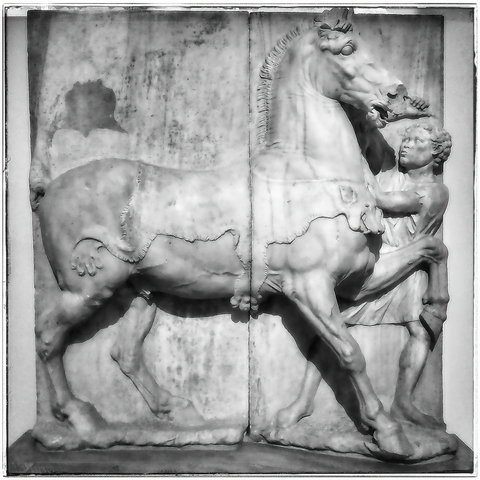
\includegraphics{smallthumb-lesson_I.jpeg}
\setfloatalignment{b}
\end{marginfigure}


\begin{abstract}
\noindent
Queste lezioni si articolano in \textsc{elementi grammaticali}, 
espressi sommariamente, seguiti da \textsc{vocabolari} per il lessico di base 
e da \textsc{frasi da tradurre} dal greco e in greco. 
\
L'approccio è quello del testo-laboratorio di morfosintassi: 
si presenta punto per punto - riprendendone la numerazione - 
l'esposizione di Gleason\cite{gleason1903}.\\
\bigskip
\noindent
Lezione XII: la declinazione in A), nomi maschili, accusativo di relazione (in originale \textit{di specificazione}), vocabolario, esercizi, lettura.
\end{abstract}

%\printclassoptions

\newthought{145. Modelli}

\begin{fullwidth}
\begin{table}[!htbp]
  \centering
  \begin{tabular}{l l l l l}
    %\toprule
	\multicolumn{5}{c}{\textsc{parole guida}} \\
	& \didobf{νεᾱνίᾱς,} & \didobf{πολίτης,} & \didobf{μαθητής,} & \didobf{σατράπης,} \\
	& \multicolumn{1}{c}{\textit{giovane uomo}}
	& \multicolumn{1}{c}{\textit{cittadino}}
	& \multicolumn{1}{c}{\textit{scolaro}}
	& \multicolumn{1}{c}{\textit{satrapo}} \\
   
	\multicolumn{5}{c}{\textsc{singolare}} \\
    \textsc{n.} & \didobf{νεᾱνίᾱς} & \didobf{πολίτης} & \didobf{μαθητής} & \didobf{σατράπης} \\
    \textsc{g.} & \didobf{νεᾱνίου} & \didobf{πολίτου} & \didobf{μαθητοῦ} & \didobf{σατράπου} \\
    \textsc{d.} & \didobf{νεᾱνίᾳ}  & \didobf{πολίτῃ}  & \didobf{μαθητῇ}  & \didobf{σατράπῃ} \\
	\textsc{a.} & \didobf{νεᾱνίᾱν} & \didobf{πολίτην} & \didobf{μαθητήν} & \didobf{σατράπην} \\
	\textsc{v.} & \didobf{νεᾱνίᾱ}  & \didobf{πολῖτα}  & \didobf{μαθητά}  & \didobf{σατράπη} \\
	
	\multicolumn{5}{c}{\textsc{plurale}} \\
	\textsc{n.v.} & \didobf{νεᾱνίαί}  & \didobf{πολῖται}  & \didobf{μαθηταί}  & \didobf{σατράπαι} \\
    \textsc{g.}   & \didobf{νεᾱνιῶν}  & \didobf{πολῑτῶν}  & \didobf{μαθητῶν}  & \didobf{σατραπῶυ} \\
    \textsc{d.}   & \didobf{νεᾱνίαις} & \didobf{πολίταις} & \didobf{μαθηταῖς} & \didobf{σατράπαις} \\
	\textsc{a.}   & \didobf{νεᾱνίᾱς}  & \didobf{πολίτᾱς}  & \didobf{μαθητάς}  & \didobf{σατράπᾱς} \\
    %\bottomrule
  \end{tabular}
  \label{tab:normaltab}
  %\zsavepos{pos:normaltab}
\end{table}
\end{fullwidth}

\newthought{Esercizi}
\begin{itemize}
\item[\textsc{1.}] In quali casi questi nomi differiscono dai nomi femminili in \didobf{α} ed \didobf{η}? 
\item[\textsc{2.}] Declina \didobf{στρατιώτης ἀγαθός, ὁ Πέρσης}.
\end{itemize}

\newthought{146.} I nomi che si riferiscono a stati/nazioni in \didobf{-ης} e i nomi in \didobf{-της} escono in \didobf{α} al \voc \si, come in \didobf{Πέρσης}, 
\textit{Persiano,} voc. \didobf{Πέρσα}; \didobf{πολίτης}, voc. \didobf{πολῖτα}. La maggior parte degli altri nomi in \didobf{-ης} escono in \didobf{η} al vocativo.

\newthought{147. Frasi Modello} da imparare a memoria.
\begin{itemize}
\item[\textsc{1.}] \didobf{ὁι πολέμιοι φοβεροὶ ἦσαν μάχην}, \textit{il nemico era terribile in battaglia.} 
\item[\textsc{2.}] \didobf{κάμνω τὴν κεφαλήν}, \textit{Ho un dolore nella (mia) testa.} 
\end{itemize}
Osserva, in textsc{1.}, che la parola \didobf{μάχην} indica in quale circostanza il nemico sia terribile; in textsc{2.} \didobf{τὴν κεφαλήν} indica la parte del corpo affetta da \didobf{κάμνω}. Questo costrutto è detto \didobf{Accusativo di Relazione (o Accusativo alla Greca).}\sidenote{\textit{Accusativo di Specificazione}, nel testo inglese.} Il costrutto si trova anche in latino (ad es. in Virgilio, \textit{nuda genu, Cressa genus}).   

\newthought{148. Regola di Sintassi.} Dopo una certa espressione (sia essa verbo, aggettivo, nome o frase) un Accusativo \textit{di Relazione} - un nome in accusativo - indica la parte o qualità alla quale l'espressione stessa \textit{si riferisce.}

\hyphenation{in-se-gnan-te}

\newthought{149. Vocabolario}

\begin{multicols}{2}
    \noindent \hangindent=1em \didobf{δείπνον, τό} \textit{cena, zuppa}.  \\
    \noindent \hangindent=1em \didobf{διδασκαλεῖον, τό} \textit{scuola}.  \\
    \noindent \hangindent=1em \didobf{διδάσκαλος, ὁ} \textit{maestro, insegnante}.  \\
    \noindent \hangindent=1em \didobf{κρόμμυον, τό} \textit{cipolla}.  \\
    \noindent \hangindent=1em \didobf{μαθητής, ὁ} \textit{scolaro}.  \\
    \noindent \hangindent=1em \didobf{νεᾱνίᾱς, ὁ} \textit{giovane uomo}.  \\
    \noindent \hangindent=1em \didobf{Ξέρξης, ὁ} \textit{Serse}.  \\
    \noindent \hangindent=1em \didobf{ὄσπριον, τό} \textit{legume,} pl. \textit{fagioli}.  \\
    \noindent \hangindent=1em \didobf{Πέρσης, ὁ} \textit{un Persiano}.  \\
    \noindent \hangindent=1em \didobf{πολίτης, ὁ} \textit{cittadino}.  \\
    \noindent \hangindent=1em \didobf{σατράπης, ὁ} \textit{satrapo,} un governatore persiano.  \\
    \noindent \hangindent=1em \didobf{στρατιώτης, ὁ} \textit{soldato}.  \\
	
	\noindent \hangindent=1em \didobf{θαυμάζω}, aor. \didobf{εθαύμασα}, \didobf{τεθαύμακα}, \textit{meravigliarsi, ammirare}. \\ 
	\noindent \hangindent=1em \didobf{μανθάνω}, aor. \didobf{ἔμαθον}, \didobf{μεμάθηκα}, \textit{imparare}. \\ 
	
\end{multicols}

\hyphenation{δι-δα-σκά-λου}

\newthought{150. Traduci:}
\textsc{1.}~\dido{οἱ δὲ πολῖται τῆς νήσου ἀγαθοὶ ἦσαν μάχην.} \quad
\textsc{2.}~\dido{τὸ τῶν στρατιωτῶν δεῖνον ἦν ὄσπρια καὶ κπόμμυα.} \quad
\textsc{3.}~\dido{τίς ἐδίδαξε τοὺς νεανίας ἐν τῷ διδασκαλείῳ;} \quad
\textsc{4.}~\dido{ἐν γὰρ τῇ τοῦ διδασκάλου οἰκίᾳ οἱ μαθηταὶ ἔμαθον γράφειν.} \quad
\textsc{5.}~\dido{Ξέρξης δὲ πέπομφε δῶρα καλὰ τῷ ἀγαθῷ σατράπῃ.} \quad
\textsc{6.}~\dido{οὐ γὰρ κακὸς ἦν μάχην, ἀλλὰ ἐστράτευτε μετὰ τῶν στρατιωτῶν.} \quad
\textsc{7.}~\dido{αἱ δὲ κόραι ἐθαύμασαν τὰς κόγχας παρὰ τῇ θύρα.} \quad
\textsc{8.}~\dido{ἐπὶ δὲ ταῖς πέτραις ηὑρήκασιν οἱ μαθηταὶ στολὰς καλάς.} \quad
\textsc{9.}~\dido{οὐ πείσεις τοὺς Πέρσας κλέπτειν τοὺς ἵππους.} \quad
\textsc{10.}~\dido{οὐκ ὥρα ἦν ἀθροίζειν τούς πολίτας.}

\newthought{151. Scrivi in Greco:}
\textsc{1.}~Chi ostacolò la vittoria dei persiani? \quad
\textsc{2.}~Le parole dei cittadini erano giuste. \quad
\textsc{3.}~Prese gli schiavi dalla fonte. \quad

\newthought{152. Armodio e Aristogitone.} (i patrioti ateniesi)\\
\dido{Ἐπεὶ δὴ ποτε \textit{(una volta)} Ἀθήωησι\sidenote{\textit{ad Atene.}} πόλεμος ἦν τοῖς ἐν τῷ
πεδίῳ πολίταις καὶ τοῖς παρὰ τῇ θαλάττῃ, Πεισίστρατός τις 
στρατιώτας ἤθροισε καὶ κατέλαβε\sidenote{\didobf{ἤρπασε}} τὴν ἄκραν τῶν Ἀθηνῶν \textit{(Atene)}.
ἀγαθὸς δὲ ἄνθρωπος ἦω καὶ σοφός, καὶ πολλοὺς ἐνιαυτοὺς \textit{(anni))}
ἔμενεν ἐν τῇ ἀρχῇ.\sidenote{legge, governo.} μετὰ δὲ τὸν θάνατον\sidenote{\textit{morte.}} 
αὐτοῦ \textit{(il suo)} οἱ υἱοὶ παρέλαβον \textit{(succeduto a)} τὴν ἀρχὴν. πρῶτον μὲν\sidenote{\didobf{πρῶτον μὲν}, \textit{all'inizio.}} καὶ οὗτοι
\sidenote{\didobf{καὶ οὗτοι,} \textit{anche loro.}} 
ἀγαθοὶ ἦσαν· ὕστερον \textit{(più tardi)} δὲ ὀλίγῳ διὰ κακόν τι δύο ωεανίαι ἐπιβουλὴν \textit{(complotto)} ἐποίησαν\sidenote{\textit{fatto, formato.}}
ἐπὶ τοὺς τυράννους \textit{(tiranni)}. τὸν μὲν Ἵππαρχον ἀπέκτειναν \textit{(messo a morte)},
Ἱππίας δέ, ὁ ἀδελγός, εὐθὺς λαβὼν\sidenote{aoristo participio attivo.} 
κατέκοψε\sidenote{\aor di \didobf{κατακόπτω}, \textit{uccidere.}} τοὺς νεανίας. ἐνταῦθα δ'ἐν ὀργῇ πολλὰ
κακὰ ἐποίησεν ὁ τύραννος. μετὰ δὲ ὀλίγους ἐνιαυτοὺς ὁι
πολῖται ἐξέβαλον αὐτὸν ἐκ τῆς χώρας. οἱ δὲ
Ἀθηναῖοι\sidenote{\didobf{οἱ τῶν Ἀθηνῶν πολῖται.}} ἔτι καὶ νῦν\sidenote{anche oggi.} λέγουσι τοῖς τέκνοις τὰ περὶ\sidenote{la storia di.}
Ἁρμοδίου καὶ Ἀριστογείτοωος, οἵ 
\center{τὸν τύραννον κτανέτην ἰσονόμους τ'Ἀθήνας ἐποιησάτην.\sidenote{che uccisero il tiranno e liberarono Atene.}}
}



\begin{figure*}[!b]
  %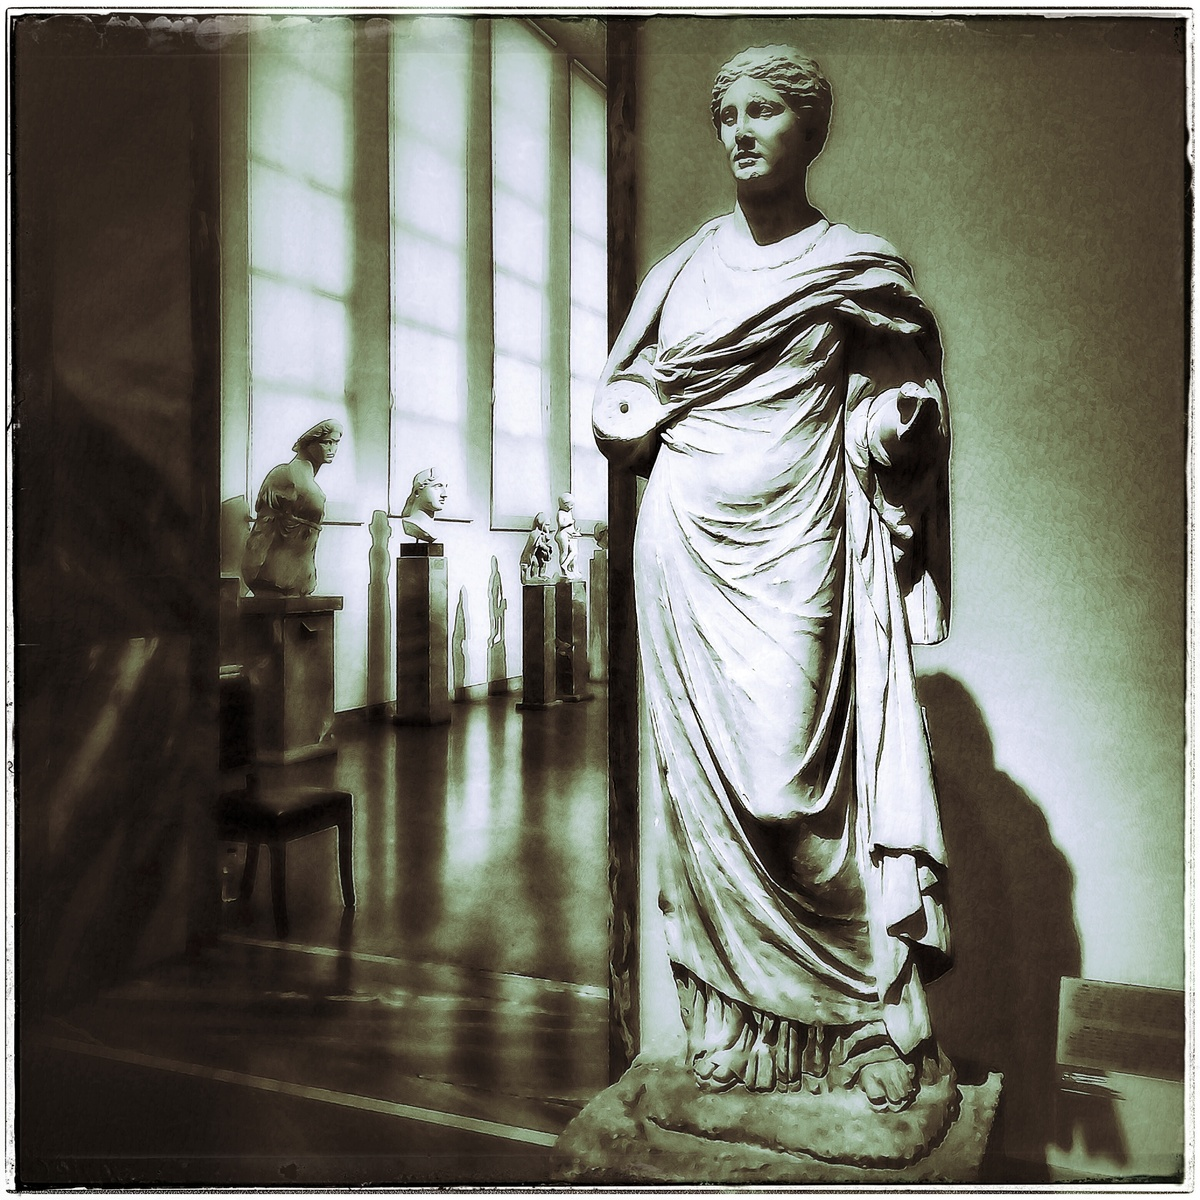
\includegraphics{thumb-lesson_XII.jpeg}
  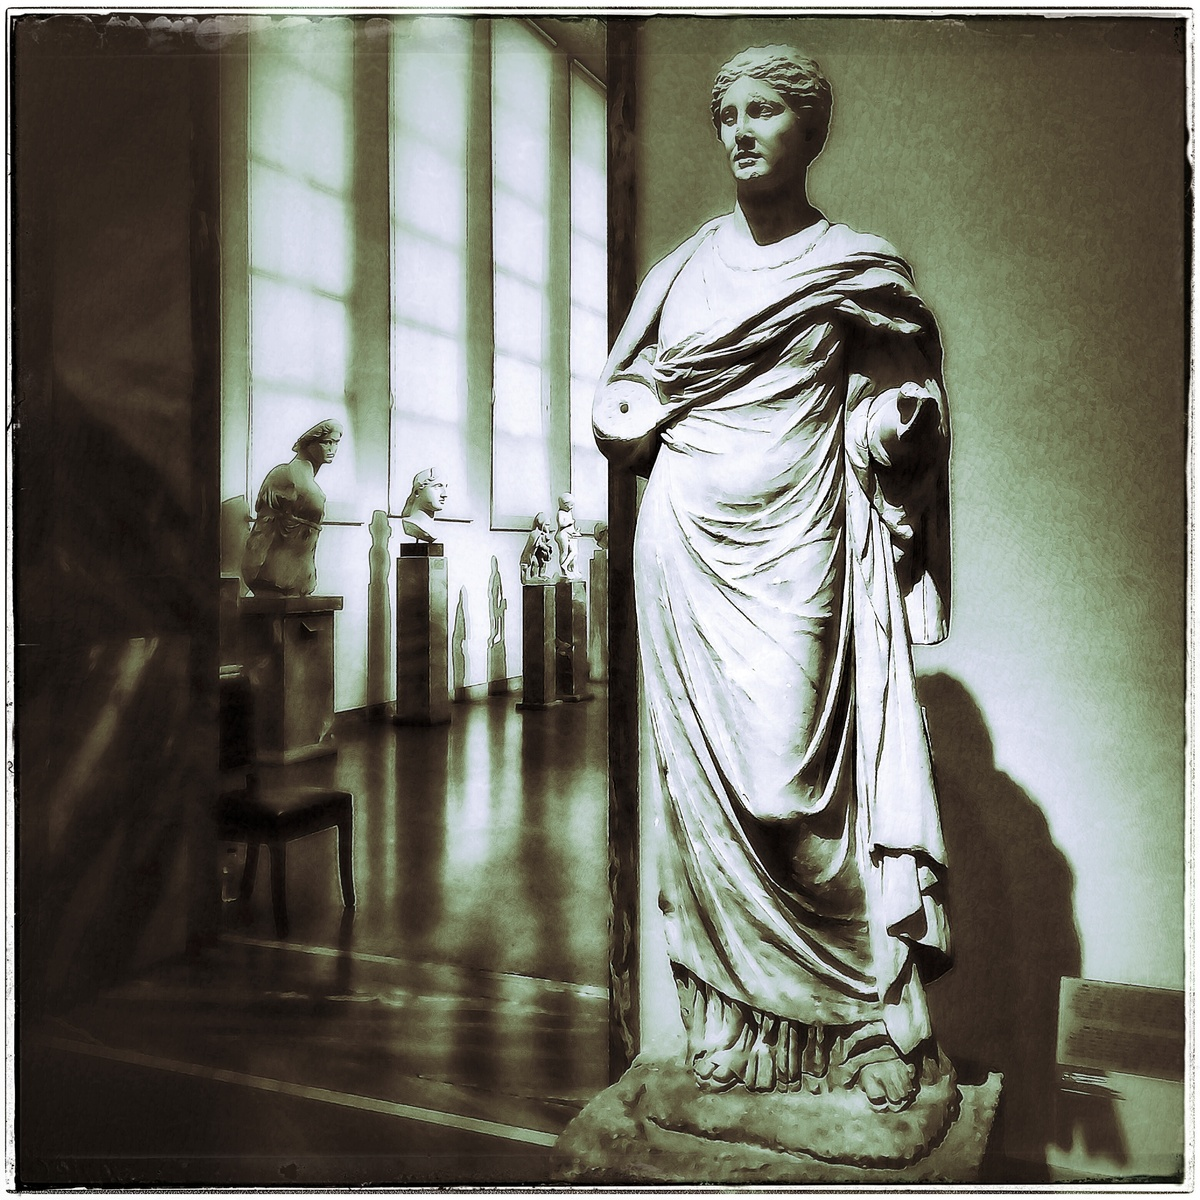
\includegraphics[width=0.9\linewidth]{thumb-lesson_XII.jpeg}
  \caption{Museo Nazionale di Archeologia di Atene}
  \label{fig:textfig}
  %\zsavepos{pos:textfig}
  %\setfloatalignment{b}
\end{figure*}

 

\nobibliography{greekBiblio}
\bibliographystyle{alpha}


\end{document}
